\section{Validation with Data from Photon Detector System Prototypes}
\label{sec:dp-pds-prototypes}

The \dword{lar} \dword{tpc} \dword{dp} proposed technology is the result of years of R\&D. From small-scale chambers to the \dword{dune} module, many prototypes have been constructed, each with some design modifications and optimizations. 
Relevant to the \dword{pds} itself, the \dword{wa105}, operated at \dword{cern} in 2017, the \dword{pddp}, under commissioning in 2019, and the \dword{dune} \dword{dpmod}, similarities and differences will be described here.

\subsection{Design Comparison between Prototypes and Far Detector System}
%Similarities and Differences
The first metric ton scale \dword{dp} \dword{lartpc}, \dword{wa105}, took cosmic data between June and November \num{2017} at \dword{cern}. 
Located \SI{1}{m} below the charge collection plane, underneath the cathode and the \dword{gg}, the \dword{pds} consisted of five \dwords{pmt} (Hamamatsu R5912-MOD20, described in more detail in Section~\ref{sec:dp-pds-photosensors}) evenly distributed along the 3$\times$1~m$^2$ area (one \dword{pmt} every \SI{50}{cm}). The demonstrator was an opportunity to test different \dword{pds} designs, particularly the \dword{tpb} coating and \dword{pmt} bases. Three \dwords{pmt} had the \dword{tpb} coating applied directly onto their windows using evaporation, but for the other two, the \dword{tpb} was deposited on a \SI{4}{\mm} thick transparent Plexiglass plate mounted on top of the \dwords{pmt}. 
While the latter solution has the advantage of being simpler and less risky to manipulate, it reduces acceptance, and possibly efficiency, because of the internal reflections between the \dword{tpb} and the Plexiglass surfaces. 
Figure~\ref{fig:pd-pds-311-pmt-tpb} shows the \dword{wa105} \dword{pds}.

\begin{dunefigure}[\dshort{wa105} \dshort{pds} ]{fig:pd-pds-311-pmt-tpb}{The \dword{wa105} \dword{pds}. Top left: \dword{pmt} with the \dword{tpb} deposited on the plexiglass plate; top right: \dword{pmt} with the \dword{tpb} coated onto the photocathode; bottom: The five \dwords{pmt} installed in the \dword{wa105} underneath the ground grid.}
%\includegraphics[width=0.25\textwidth]{graphics/dppd_PMTPlate}
%\includegraphics[width=0.33\textwidth]{graphics/dppd_PMTTPB.jpeg}\\
%\includegraphics[width=0.6\textwidth]{graphics/dppd_PMT_311_installation.jpg}
\includegraphics[width=0.5\textwidth]{dppd_311_PMT_combined}
\end{dunefigure}

Two power supply polarities were used. Three \dwords{pmt} were equipped with a negative \dword{hv} base, i.e., a negative bias voltage was applied to the photocathode, and the anode was grounded. This system required two cables: one for the \dword{hv} system and one for the signal. A positive base served the other two \dwords{pmt}: a single cable positively biased the anode and carried the signal, and the cathode was grounded. The \dword{hv} and the signal were then externally decoupled using a splitter (see Section~\ref{sec:fddp-pd-4.2}). The latter design has the advantage of reducing the number of feedthroughs and cables while also reducing the noise. Overall, four configurations were tested (see Table~\ref{tab:dp-pds-311conf}). During the \dword{wa105} operation, the \dwords{pmt} operated at a fairly %rather 
uniform gain of approximately \num{e6} with a readout sampling of \SI{250}{MHz}.

\begin{dunetable}
[\dshort{wa105} \dshort{pmt} configurations.]
{cccccc}
{tab:dp-pds-311conf}
{Configuration of the five \dwords{pmt} installed in the \dword{wa105}.}
\dword{pmt} & Base & Coating & Voltage (kV) & Gain (\num{e6}) & Noise (ADC)\\ \colhline
%\hline
1 & Negative & Coating & \num{-1.2} & 0.92$\pm$0.13 & \num{0.7} \\ \colhline
2 & Negative & Plate   & \num{-1.2} & 1.01$\pm$0.12 & \num{0.7} \\ \colhline
3 & Positive & Coating & \num{1.1} & 0.95$\pm$0.11 & \num{0.4} \\ \colhline
4 & Positive & Plate   & \num{1.1} & 1.26$\pm$0.15 & \num{0.4} \\ \colhline
5 & Negative & Coating & \num{-1.2} & 1.33$\pm$0.15 & \num{0.8} \\
%\hline
\end{dunetable}

In \dword{pddp}, \num{36} \dwords{pmt} are installed \SI{6}{\m} below the collection plane, again underneath the cathode and the \dword{gg}. The \dword{pmt} density is lower than in the \dword{wa105}. Their positioning over the \SI{36}{m$^2$} area was optimized with simulations. The number of \dwords{pmt} is higher around the center of the active volume and lower near the \dword{fc} borders. This positioning maximizes the amount of light collected from cosmic rays.

After evaluating the demonstrator configurations, the \dword{tpb} was directly evaporated onto the \dword{pmt} windows, and the \dword{pmt} base was chosen to have positive polarity. This configuration maximizes collection efficiency and reduces both the number of cables and the electronic noise. 

For the \dword{dpmod} \dword{pds}, \dword{tpb} is directly applied to the \dword{pmt} windows, and the positive biasing scheme is implemented. The aspect ratio between cathode size and drift distance is larger than in \dword{pddp}, so the amount of light loss by absorption on the \dword{fc} should be smaller. Therefore, the \dword{dpmod} \dword{pds} layout should be uniform, with \dwords{pmt} on a regular lattice spaced every \SI{1.02}{m}. 

%%%%%%%%%%%%%%%%%%%%%%%%%%%%%%%%%%%%%%%%%%%%%%%%%%%%%%%%%%%%%%%%%%%%

\subsection{WA105 Light Data Results and Simulation Validation}

Analysis of data taken during the \dword{wa105} operation provides the first validation of and improvements in the light simulation developed so far. 
The demonstrator ($3\times1\times1$~m$^3$ active volume) has linear dimensions comparable with the Rayleigh scattering length, which is approximately \SI{60}{\cm}. 
As a consequence, the light absorbed by elements of the detector (such as the \dword{fc}, \dword{lem}, or cathode) may become a problem.
Hence, light maps were created with particular care for precision in reproducing the demonstrator's geometry.

Two triggering schemes were used during the \dword{wa105} operation.
The first was provided by an external muon tagger, the \dword{crt}, to record horizontal muons. The \dword{crt} was made of plastic scintillator planes on each side of the detector.
The second was provided by the \dwords{pmt} themselves, requiring that the five sensors record sufficient light in coincidence. In this configuration, the system recorded more vertical muons and showers.

Using the \dword{crt} trigger condition, a rough track reconstruction is possible because the \dword{crt} provides coordinate information with \SI{11}{\cm$^2$} resolution. Hence, even without charge information, as for data taken at null field, it is possible to select muon-like tracks and retrieve the shortest distance between the track and each \dword{pmt}. A schematic drawing of the \dword{wa105} detector is presented in Figure~\ref{fig:pd-pds-311schema} with the relevant track parameters.

\begin{dunefigure}[\dshort{wa105} schematic drawing]{fig:pd-pds-311schema}{Schematic view of the \dword{wa105}. 
The fiducial volume is in gray and limited from the collection plane area to the cathode. The active volume is in yellow. Its volume is defined by the collection plane: the \dword{fc} to the top of the \dwords{pmt}. A track that would be detected by the \dword{crt} is shown with its minimum distance to \dword{pmt} \num{3} in red.}
\includegraphics[width=0.75\textwidth]{graphics/dppd_7_2_v2}
\end{dunefigure}

From the \dword{pds} point of view, the \dword{wa105} operation lasted several months since light was also collected during the \cooldown, fill, and commissioning stages of the demonstrator.
The \dword{pds} performed with high stability during this entire period. 
In Figure~\ref{fig:pd-pds-311-ped}, the  pedestal \dword{rms} is shown for one positive and one negative base \dword{pmt} as a function of time for \num{5} months of operation. 

\begin{dunefigure}[\dshort{wa105} \dshort{pmt} pedestal \rms]{fig:pd-pds-311-ped}{Pedestal \dword{rms} for one negative base \dword{pmt} (black) and one positive base \dword{pmt} (red) between July and December 2017 during the operation of the \dword{wa105}.}
\includegraphics[width=0.9\textwidth]{graphics/dppd_311_pedestal_rms.pdf}
\end{dunefigure}

Figure~\ref{fig:pd-pds-311-LAr-GAr} shows the average waveforms for \dword{pmt} 5 in gas and liquid argon with no drift field. These waveforms are fitted with a Gaussian to describe the response function, and convoluted with a sum of three exponentials to describe the fast, slow, and intermediate components. 
The extracted values agree with the literature, although the lifetime of the fast component has been fixed at \SI{6}{ns} in the fitting procedure.

\begin{dunefigure}[GAr and LAr scintillation profile in the \dshort{wa105}]{fig:pd-pds-311-LAr-GAr}{Scintillation time profile in the absence of drift field recorded in GAr (left) and LAr (right) in black. In red, the fit performed with a sum of three exponentials (describing the fast, intermediate, and slow components, all shown as dotted blue lines) convoluted with a gaussian to take into account the response function of the \dword{pmt}. The intermediate component improves the fit quality considerably although a consensus on its interpretation is not reached in the community at this moment. The extracted lifetimes are shown in the figure.}
\includegraphics[width=0.85\textwidth]{graphics/dppd_311_lar_gar_fit.pdf}
\end{dunefigure}

Many studies show that $\tau_{slow}$, the slow component lifetime (Section~\ref{sec:dp-pds-overview_scintillation}) is very sensitive to the amount of impurities in the liquid.
To monitor the purity of the \dword{lar} as a function of time, the same fit has been performed on several runs under similar conditions. 
Figure~\ref{fig:pd-pds-311-purity} presents the evolution of $\tau_{slow}$ for \SI{15}{days} of operation.
The results exhibit a very stable amount of impurity, which agrees with the stability of the electron lifetime measured using the charge collection.

\begin{dunefigure}[Evolution of $\tau_{slow}$ as a function of time in the \dshort{wa105}]{fig:pd-pds-311-purity}{Evolution of $\tau_{slow}$ over \num{15} days of operation of the \dword{wa105}. The points are the averages over the values extracted from the fits to the waveforms of the three negative base \dwords{pmt} for runs taken with no drift field. Preliminary results.}
\includegraphics[width=0.7\textwidth]{graphics/dppd_311_purity.pdf}
\end{dunefigure}

The S2 light has also been recorded in dedicated runs using a \SI{1}{ms} recording time window.
Figure~\ref{fig:pd-pds-311-S2} shows the average waveforms from runs with a drift field of \SI{0.5}{kV/cm} and an extraction field of \SI{2}{kV/cm} (\SI{3}{kV/cm}) in liquid (gas). In the figure, one run has no amplification field, the others have the \dwords{lem} polarized to provide an amplification field of \SI{25.5}{kV/cm}. 
The effect of the \dwords{lem} on the amount of S2 light generated is clear: 
the S2 light extends for about \SI{600}{$\mu$s} after emission of the prompt signal, agreeing with the electron drift time over \SI{1}{m} in such a drift field.

\begin{dunefigure}[S2 light at different amplification field in the \dshort{wa105}]{fig:pd-pds-311-S2}{Average waveforms of negative based \dwords{pmt} in a \SI{1}{ms} window. Both runs were taken with a drift field of \SI{0.5}{kV/cm} and an extraction field of \SI{3}{kV/cm} in gas. The S2 light extends for about \SI{600}{$\mu$s}, as expected.}
\includegraphics[width=0.7\textwidth]{graphics/dppd_311_S2_extraction.pdf}
\end{dunefigure}
Using data taken at null field in \dword{crt} triggering mode, muon-like tracks are selected. Further, the tracks must cross the active volume for distances longer than \SI{3.1}{\m}. 
The S1 charge collected by each \dword{pmt} is calculated by integrating the \dword{adc} values in a \SI{1}{\us} window starting from the S1 peak; this charge value is then converted into the number of detected \dwords{pe} using the calibrated \dword{pmt} gains in Table~\ref{tab:dp-pds-311conf}.

In the simulation, \SI{4}{\GeV} muons are generated from one \dword{crt} panel to the other with data-driven kinematics. The number of \dwords{pe} collected by each \dword{pmt} is generated according to the light maps. To suppress spurious triggers, data analysis uses a selection of the minimum amount of light recorded by all \dwords{pmt}; this does not apply to \dword{mc}. Moreover, the \dword{pmt} signal must not saturate the readout %only 
for data analysis but not for \dword{mc}. Figure~\ref{fig:dp-pds-311charge} compares the number of \dwords{pe} collected in data analysis and in \dword{mc}. The data and \dword{mc} agree well with one another. 

In the \dword{wa105}, the \dword{pmt} gain was adjusted so that S1 and S2 light could be seen, thus increasing the trigger rate while minimizing the \dword{pmt} \dword{adc} saturation. 
In the \dword{dpmod}, the situation will be different as the volume is much larger and part of the triggering modes will be independent of the \dwords{pmt}. 
The \dword{pmt} gain will therefore be adjusted accordingly and the events saturating the \dword{adc} should not be as problematic as it could have been in the \dword{wa105}.
%\fixme{Give more details about why \dword{pmt} saturation in \dword{wa105}, and why this is not worrisome in \dpmod?}

\begin{dunefigure}[Charge collected in the \dshort{wa105} vs \dshort{mc}]{fig:dp-pds-311charge}{ Charge collected by the \dwords{pmt} in a \SI{1}{\us} window containing the S1 peak for muon-like tracks triggered by the \dword{crt} panels. The data is shown in black and the simulation in red. The distributions are normalized to unity for clarity. Preliminary results.}
\includegraphics[width=0.95\textwidth]{graphics/dppd_311_charge_mc_v2.pdf}
\end{dunefigure}

\begin{dunefigure}[Charge collected vs track-PMT shortest distance]{fig:dp-pds-311profile}{Profile histograms of charge collected as a function of the track-PMT shortest distance. The data is in black, the simulation in red. Preliminary results.}
\includegraphics[width=0.95\textwidth]{graphics/dppd_311_charge_dist_mc.pdf}
\end{dunefigure}

%\fixme{This is rather distance vs charge. Is it possible to swap the x and y axis and reproduce the plots?}

The \dwords{pe} collected per \dword{pmt} depends strongly on the shortest track-\dword{pmt} distance. Many factors can affect how much charge is collected, primarily, the scattering length, also known as the Rayleigh scattering length. This quantity is still subject to debate among the \dword{lar} community because its measurement is fairly complicated. Current estimates of the scattering length range from \SI{20}{\cm} to \SI{1}{\m}.
In the \dword{wa105} simulation, the scattering length was set to L$_{ray}$ = \SI{55}{\cm}.
Figure~\ref{fig:dp-pds-311profile} shows the charge collected as a function of the shortest track-\dword{pmt} distance in the form of profile histograms. The overall trend is very similar for data and \dword{mc}, also across all the \dwords{pmt}. However, the profile histogram slopes indicate that the assumed scattering length in \dword{mc} could be better tuned to reproduce the data, e.g., toward larger values of the Rayleigh scattering length.

%%%%%%%%%%%%%%%%%%%%%%%%%%%%%%%%%%%%%%%%%%%%%%%%%%%%%%%%%%%%%%%%%%%%

\subsection{Installation of the \dshort{pddp} Photon Detector System}

\dword{pddp} \dword{pds} installation was smooth as it followed the planned procedures. As a result, no incidents were reported and all \dwords{pmt}, cables and fibers operate as expected. Important lessons from \dword{pddp} have been learned from this installation; % of the \dword{pddp} \dword{pds}. T
they are summarized below. Figure~\ref{fig:dppd_pmt_installation} shows the placement of the \num{36} \dwords{pmt} in \dword{pddp} on the cryostat floor, performed in February 2019.

\begin{dunefigure}[Installation of the \dshort{pddp} PDS]{fig:dppd_pmt_installation}{Photon detector system installed in \dword{pddp}.}
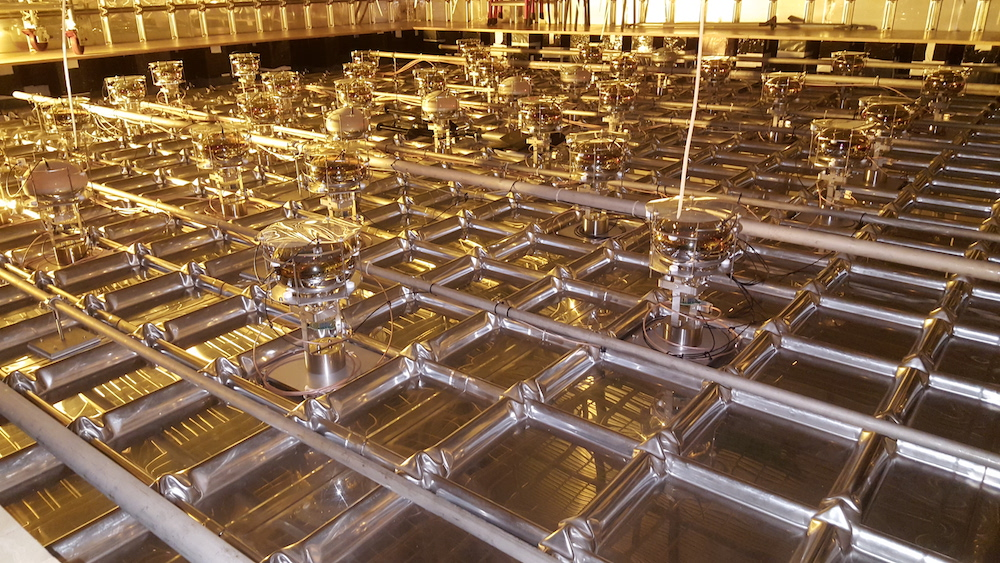
\includegraphics[width=0.8\textwidth]{graphics/dppd_pmt_installation.jpg}
\end{dunefigure}

One of the most important aspects of the installation is the order of the tasks. Since the \dword{pddp} \dword{pds} installation activities lasted several days, % in the \dword{pddp} case, 
and will last several months for a \dword{dpmod}, and given that other persons have to work near the \dword{pds} components, the risk of damage has to be considered. The fragility of the components determines the installation order. The \dword{pmt} supporting bases, the signal-HV \dword{pmt} cables and calibration fibers must be be installed first, then the \dwords{pmt} can be mounted on their holders and connected to the cables and fibers. The need to protect the installed components has to be evaluated if subsequent activities take place around them. For example,  temporary protective plates were placed in front of the \dword{pddp} \dword{pmt} photocathodes, and the \dword{pmt} units were enclosed in temporary plastic bags. 

In \dword{pddp}, the \num{36} \dwords{pmt} are divided into \num{2} symmetric groups of 18 whose cables and fiber go to different output chimneys (CF250). Inside the cryostat, the \dwords{pmt} are separated in six groups of six each. This arrangement simplified the installation of the calibration fibers, given that each fiber bundle has seven fibers (six plus one spare). We have conceptually divided the \dword{dpmod} \dword{pds} into several sectors. \fixme{how many?}

Concerning organizational matters, \dword{pddp} experience shows that several documents should be prepared prior to installation, including a detailed description of all the tasks to be performed, a time estimation for all of them, and a list of the necessary items. In addition, the required status of the detector before each installation stage should be indicated. This information must be as detailed as possible so that %. The benefits of a detailed planning are:

\begin{itemize}
\item all the persons participating in the \dword{pds} installation know their roles,
\item the required material is %foreseen and is 
available when needed,
\item the interaction with other installation crews is planned,
\item the expected time for the installation is known in advance and extra time for unexpected events can be added,
\item it is possible to communicate beforehand all the requests to the coordinator of the installation, and
\item the overlapping of activities and the waiting times are minimized. 
\end{itemize}

In June 2019, the wavelength-shifter on 30 \dwords{pmt} for \dword{pddp} was changed from evaporated \dword{tpb} to a sheet of polyethylene naphthalate (PEN), which was placed on top of each \dword{pmt} to compare the performance of the different wavelength-shifter techniques. Since the \dwords{pmt} were already installed, the operation took place in situ before closing the cryostat. \fixme{This feels unconnected; relate this to planning: was this planned, or in response to an event? Did it interfere with other things? Anne}

%%%%%%%%%%%%%%%%%%%%%%%%%%%%%%%%%%%%%%%%%%%%%%%%%%%%%%%%%%%%%%%%%%%%

\subsection{Preliminary Performance of the \dshort{pddp} Photon Detector System}

During summer 2019, the \dword{pddp} cryostat was closed, purged with argon gas, and filled with \dword{lar}. Light data taking started %already when 
as soon as the argon gas filled the detector and of course continued once it was filled with  \dword{lar}. See scintillation light event examples for both cases in Figure~\ref{fig:pd-pds-gas-liquid}. As of this writing, all 36 \dwords{pmt} have been operational since the beginning and data are being taken under different conditions.

\begin{dunefigure}[\dshort{pddp} scintillation light events in argon gas and \dshort{lar}]{fig:pd-pds-gas-liquid} {Examples of scintillation light events in one \dword{pmt} of \dword{pddp} when the detector was filled with gas argon (left) and with \dword{lar} (right). The different time profile of scintillation light production in the two cases is clearly visible.}
\includegraphics[width=0.45\textwidth]{graphics/dppd_gas.png}
\includegraphics[width=0.45\textwidth]{graphics/dppd_liquid.png}
\end{dunefigure}
%%%% anne to here 10/19

The \dword{pmt} gains are calculated regularly with the light calibration system. \dwords{pmt} are individually illuminated at the \dword{spe} level, and gain versus \dword{pmt} \dword{hv} curves are obtained. Figure~\ref{fig:pd-pds-gain} shows the gain evolution at a given \dword{hv} for calibrations performed once the detector was fully filled with \dword{lar}. It has to be noted that \dwords{pmt} are biased off between measurements and gain shifts of 21\% are expected \cite{Belver:2018erf}. When gain shifts are detected, \dword{hv} values are modified so that \dwords{pmt} keep operating at the same gain. \dwords{pmt} usually work at 10$^7$ gain and dedicated measurements at lower gains are also taken.

\begin{dunefigure}[\dshort{pddp} gain evolution]{fig:pd-pds-gain} {\dword{pmt} gain evolution in \dword{pddp} at a given \dword{hv} for five \dwords{pmt} during the first month of commissioning.}
\includegraphics[width=0.5\textwidth]{graphics/dppd_gain.pdf}
\end{dunefigure}

Various trigger possibilities have been tested with the \dword{pddp} \dword{pds}. First, it is possible to trigger with the light calibration system, as explained before, and also take random trigger data inhibiting the \dwords{led}. Second, commissioning data are usually taken in the \dword{pmt}-self trigger mode selecting the \dwords{pmt} that enter in the trigger and the number of \dwords{pmt} required to trigger. Last, the global \dword{daq} trigger integrating the \dword{wr} system has been tested with random triggers.

Different data analyses are ongoing, and some preliminary information on the \dword{pddp} \dword{pds} performance is presented here. Figure~\ref{fig:pd-pds-S1} shows a scintillation light event example as detected in the four central \dwords{pmt}. This particular event is recorded in the absence of \efield{}s (only S1 signal is expected) with \dword{pmt}-self trigger on \dword{adc} channel 20. The goal of this run was to monitor the \dword{lar} purity, and a slow component lifetime of $\tau_{slow}$=\,(1.46\,$\pm$\,0.2)\,$\mu$s is obtained from the average waveform fit. The two \dwords{pmt} shown at the top (\dword{adc} channels 20 and 21) are coated with \dword{tpb}, while the two shown at the bottom (\dword{adc} channels 22 and 23) have PEN sheets as wavelength shifter. A preliminary analysis shows that the average S1 amplitude for the \dwords{pmt} using PEN is 15\% of the amplitude of the \dwords{pmt} coated with \dword{tpb}. The low noise in the baseline is remarkable, as the pedestal STD is less than one \dword{adc} count. \fixme{what is STD?}

\begin{dunefigure}[\dshort{pddp} S1 event examples]{fig:pd-pds-S1} {\dword{pddp} event example of the four central \dwords{pmt}. This run is taken without \efield{}s with \dword{pmt}-self trigger on \dword{adc} channel 20. The two \dwords{pmt} shown in the top are coated with \dword{tpb}, while the two shown in the bottom have a PEN sheet as wavelength shifter. Data are taken with the V1740 CAEN ADC using a \SI{16}{ns} sampling rate. Values for each waveform of the total integrated charge, minimum amplitude, and baseline are given.}
\includegraphics[width=0.75\textwidth]{graphics/dppd_S1.png}
\end{dunefigure}

Data with fields (drift, extraction and amplification) have also been taken during the commissioning phase. Figure~\ref{fig:pd-pds-S2} shows an event example for the four central \dwords{pmt} acquired with the \dwords{tpc} operated at a drift field of \SI{50}{kV} and extraction fields of \SI{6.1}{kV}. The secondary scintillation light (S2) from the electroluminescence of the electrons extracted in the argon vapor (more than \SI{6}{m} far away from the \dwords{pmt}) is observed in all \dwords{pmt}.

\begin{dunefigure}[ProtoDUNE-DP S2 event examples]{fig:pd-pds-S2} {\dword{pddp} event example of the four central \dwords{pmt}. %The run is taken with the TPC operated at a drift field of 0.5 kV/cm and extraction fields of 6.1 kV.
This run is taken with the drift and extraction fields turned on. %The y-axis has been zoomed, so the S1 signal is cut to focus on the S2 signal that lasts hundreds of $\mu$s.
%The y-axis has been zoomed in order to focus on the S2 signal that lasts hundreds of $\mu$s.
The $y$-axis was zoomed in order to focus on the S2 signal that lasts hundreds of $\mu$s and the $x$-axis was rebinned for better visibility.}
\includegraphics[width=0.75\textwidth]{graphics/dppd_S2.png}
\end{dunefigure}
